\textbf{COLUNI 2026 -- Questão 18}\par\medskip As amigas Juliana e Mayume partiram da casa da Juliana, com destino à escola que estudam. Enquanto Mayume foi direto para a escola, Juliana, primeiro passou pelo correio, e depois seguiu para a escola. Considere que as localidades indicadas na figura “Casa da Juliana”, “Correio” e “Escola” e os trajetos percorridos pelas amigas sejam, respectivamente, os vértices e os lados de um triângulo retângulo.

% COLUNI-AUTO-FIGURES-BEGIN
\begin{figure}[htbp]
\centering
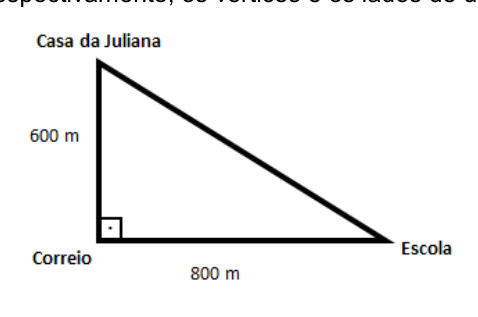
\includegraphics[width=0.55\linewidth]{static/simulados/coluni/figuras/2026/questao-18/figura-1.png}
\end{figure}
% COLUNI-AUTO-FIGURES-END

De acordo com os dados apresentados, a distância percorrida por Juliana foi maior que a distância percorrida por Mayume em:
\begin{enumerate}
\item 30\%.
\item 35\%.
\item 40\%.
\item 45\%.
\end{enumerate}
